\section{Experiment 9A: learned compatibility groups}
\label{sec:experiment9a}

\paragraph{Question.}
Experiment 9A asks whether useful sharing groups and their number can be learned
from compact local LPV estimates rather than supplied as oracle family labels.
It is deliberately non-private: privacy-aware cluster sizing and protection of
cluster discovery are deferred until useful grouping itself passes a hard gate.
Training vehicles determine the partition and cluster models; separate unseen
vehicles are assigned by their local three-ratio estimate. Simulator family
labels enter only the oracle baseline and post-hoc adjusted Rand index (ARI).

\paragraph{Methods and frozen selection.}
Ten fresh fleets (seeds 116--125) contain 60 training and ten unseen test
vehicles per simulated family. All clients receive three one-second,
single-speed records. The methods are Local (30 test-vehicle models), Global
(one model), Oracle family (three models), ordinary $K$-means with fixed $K=3$,
and two learned-$K$ variants. Parameter clustering operates on publicly bounded
normalized log-ratios. Control clustering multiplies all clients by one public,
label-independent diagonal metric derived at the nominal public plant; it does
not use family-specific weights.

Learned $K$ maximizes training silhouette over $K\in\{2,\ldots,8\}$, subject to
at least ten training clients per cluster. If no candidate exceeds 0.25, the
method selects $K=1$. Unseen assignments use the nearest training centroid.
The hard gate requires learned-$K$ control clustering to track no worse than the
oracle-family model, remain amplitude-feasible with frozen radius below one,
and deploy fewer models than Local.

\begin{table}[htbp]
\centering
\caption{Experiment 9A unseen-client results.}
\label{tab:experiment9a-results}
\begin{tabular}{lrrrr}
\toprule
Method & Tracking & Models & Parameter error & Worst client\\
\midrule
Local & 0.006692 & 30.0 & 0.0230 & 0.007397\\
Global & 0.011700 & 1.0 & 0.1299 & 0.018969\\
Oracle family & 0.007556 & 3.0 & 0.0469 & 0.010510\\
Fixed $K=3$ & 0.007554 & 3.0 & 0.0469 & 0.010500\\
Learned-$K$ parameter & 0.007554 & 3.0 & 0.0469 & 0.010500\\
Learned-$K$ control & 0.007757 & 2.9 & 0.0497 & 0.011256\\
\bottomrule
\end{tabular}
\end{table}

\begin{table}[htbp]
\centering
\caption{Learned partition diagnostics averaged over ten fleets.}
\label{tab:experiment9a-clusters}
\begin{tabular}{lrrrr}
\toprule
Method & $K$ range & Train ARI & Test ARI & Silhouette\\
\midrule
Fixed $K=3$ & 3--3 & 0.987 & 1.000 & 0.537\\
Learned-$K$ parameter & 3--3 & 0.987 & 1.000 & 0.537\\
Learned-$K$ control & 2--3 & 0.915 & 0.951 & 0.572\\
\bottomrule
\end{tabular}
\end{table}

\begin{figure}[htbp]
\centering
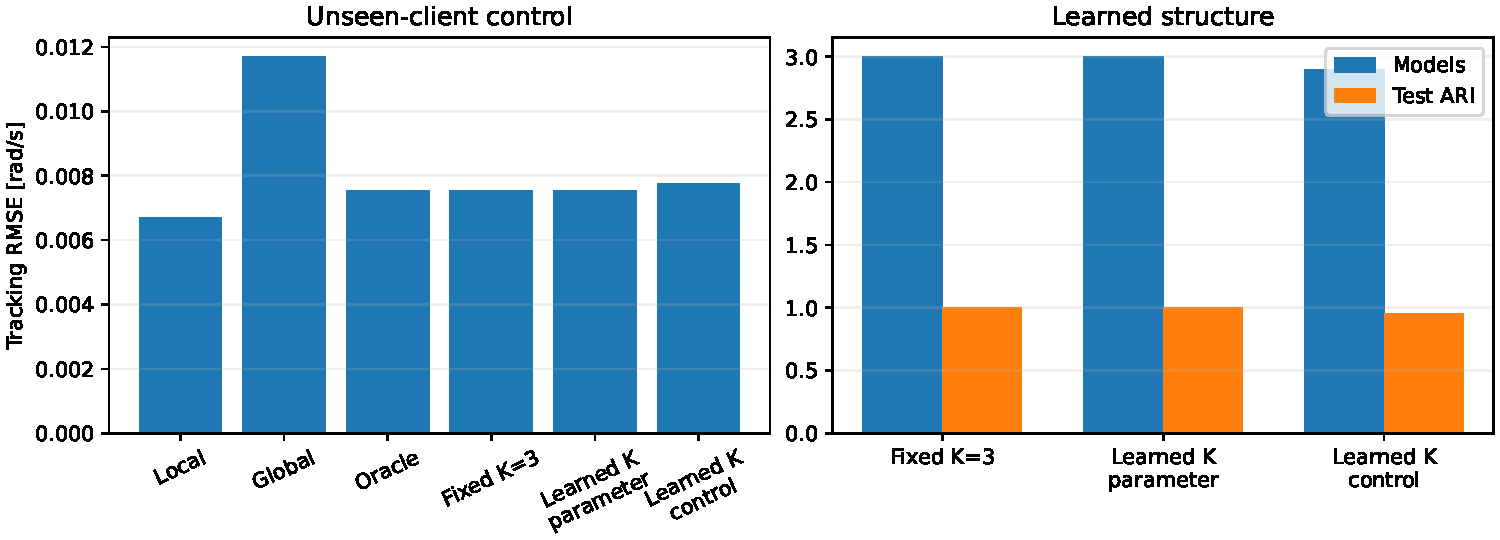
\includegraphics[width=0.93\linewidth]{../results/figures/experiment_9a_learned_groups.pdf}
\caption{Unseen-client tracking and learned grouping structure in Experiment
9A. ARI is diagnostic only and is not used for model selection.}
\label{fig:experiment9a}
\end{figure}

\paragraph{Results.}
All 2,100 local fits converge and all 5,400 nonlinear evaluations are
amplitude-feasible with frozen radius below one. Learned-$K$ parameter
clustering selects three groups in every fleet. Its training ARI is 0.987, while
nearest-centroid assignment reaches test ARI 1.0 on all unseen vehicles. Its
tracking RMSE, 0.007554 rad/s, is effectively equal to and slightly below the
oracle-family value of 0.007556 rad/s. It therefore removes the label assumption
for this discrete-family benchmark while retaining three deployed controllers
instead of 30 Local controllers. Local remains 11.4\% better in tracking, and
Global is 54.8\% worse than oracle family.

The learned-$K$ control variant fails the hard gate. It chooses $K=2$ on seed
124, merges incompatible groups (test ARI 0.506), and increases that fleet's
tracking error by 25.5\% relative to oracle. Across all fleets it is 2.66\%
worse than oracle. Its higher silhouette shows why geometric compactness alone
is insufficient: the public curvature used to allocate DP noise suppresses a
parameter direction that remains important for deciding which clients should
share a controller.

\paragraph{Decision and limitations.}
Experiment 9A supports label-free parameter-space compatibility discovery, but
rejects direct reuse of the control-aware privacy geometry for clustering. The
positive result is presently limited by the simulator's clearly discrete three-
family construction. Before it becomes a strong paper contribution, Experiment
9B must test shorter/noisier identification, unbalanced populations, and
continuous heterogeneity. Moreover, the server currently observes individual
local estimates; this is trusted-server clustering, not end-to-end private
group discovery. Privacy-aware clustering should proceed only if 9B confirms
stable useful partitions beyond this favorable discrete setting.

\paragraph{Reproducibility.}
The frozen protocol is in \path{code/config/experiment_9a.json}; implementation
is in \path{code/experiments/experiment_9a_learned_groups.py}. Seed summaries,
candidate scores, selected-cluster diagnostics, and conclusions are retained
under \path{results/tables}.
